\documentclass{beamer}
\usetheme{Madrid}
\usepackage{mathtools}
\usepackage{graphicx}
\usepackage[scaled]{beramono}
\usepackage{listings}

% Custom colors
\usepackage{color}
\definecolor{deepblue}{rgb}{0,0,0.5}
\definecolor{deepred}{rgb}{0.6,0,0}
\definecolor{deepgreen}{rgb}{0,0.5,0}

\title{Asian Option Pricing through Finite Difference Schemes}
\author{Emmanuel Goh}
\date{\today}

\begin{document}

  \begin{frame}
    \titlepage
  \end{frame}

  \begin{frame}
    \frametitle{Outline}
    \tableofcontents
  \end{frame}

  \section{Recap}
  \begin{frame}
    \frametitle{Recap}
    The purpose of this project was to model 5 different Partial Differential Equations governing the price of Asian Options, based on a previous paper which highlighted certain similarities between the different equations
  \end{frame}

  \section{Definitions}
  \begin{frame}
    \frametitle{Definitions}
    \begin{table}[h]
    \begin{tabular}{|c|c|}
      \hline
      \textbf{Description} & \textbf{Variable Name} \\ \hline
      Stock Price & \(S\) \\
      Strike Price & \(K\)\\
      Average Price & \(A\) \\
      Time ago which averaging started & \(t_0\) \\
      Remaining lifespan of the Option & \(T\) \\
      Risk Free Rate & \(r\) \\
      Dividend Rate & \(\delta\) \\
      \hline
    \end{tabular}
    \caption{Variables used in various equations}
    \label{table:name}
    \end{table}
  \end{frame}

  \begin{frame}
    \frametitle{Definitions}
    The average price of a stock is given by
    \begin{equation}
      A_T = \frac{t_0A + \int_0^T S_t \mathrm{d}t}{t_0 + T}.
    \end{equation}

    We also define
    \begin{equation}
      \xi_t =
      \begin{dcases*}
        a(t) + b(t) \frac{A_t - Ke^{-\delta(T-t)}}{\tilde{S_t}} & Fixed calls (in general) \\
        a(t) + b(t) \frac{A_t}{S_t} & Floating calls (in general)
      \end{dcases*}
    \end{equation}
  \end{frame}

  \begin{frame}
    \frametitle{Definitions}
    We define also the function \(q(t)\) such that
    \begin{equation}
      q(t) =
      \begin{dcases*}
        \frac{1 - e^{-(r-\delta)(T-t)}}{(r-\delta)(t_0 + T)} & \(r \neq \delta\) \\
        \frac{T-t}{t_0 + T} & \(r\) = \(\delta\)
      \end{dcases*},
    \end{equation}
    and by this we obtain the value process of a self-financing portfolio with payoff \(A_T\), also known as the average asset.

    \begin{equation}
      A_t = e^{-r(T-t)}E_P(A_T|\mathcal{F}_T) = q(t)\tilde{S_t} + e^{-r(T-t)} \frac{t_0 A + \int_0^tS_u\mathrm{d}u}{t_0+T}.
    \end{equation}
  \end{frame}

  \section{Partial Differential Equations}

  \begin{frame}
    \frametitle{Partial Differential Equations}
    We have the generic partial differential equation that governs the option price given as
    \begin{equation}
      \phi_t + [\dot{a}(t) + \dot{b}(t)(\xi - a(t))/b(t)]\phi_\xi + \frac{1}{2}\sigma^2[a(t)+b(t)q(t) - \xi]^2\phi_{\xi\xi} = 0,
    \end{equation}
    where \(\phi(T, \xi) = f(\xi)\), and \(f(\xi)\) is defined as per the below table.

    \begin{table}[h]
      \begin{tabular}{|c|c|c|}
        \hline
        & Fixed Strike & Floating Strike \\
        \hline
        Calls & \(max\{(\xi - a(T))/b(T), 0\}\) & \(max\{(a(T) - \xi)/b(T) + 1, 0\}\) \\
        Puts & \(max\{(a(T) - \xi)/b(T ), 0\}\) & \(max\{(\xi - a(T))/b(T) - 1, 0\}\)\\
        \hline
      \end{tabular}
      \caption{Different possible values of \(f(\xi)\)}
    \end{table}
  \end{frame}

  \begin{frame}
    \frametitle{Boundary Conditions}
    \begin{table}[h]
      \begin{tabular}{|c|c|c|}
        \hline
        & \(\xi \rightarrow \infty\) & \(\xi \rightarrow -\infty\) \\
        \hline
        \(b(t) > 0\) &  & \(\phi(t, \xi) \rightarrow 0\) \\
        \(b(t) < 0\) & \(\phi(t, \xi) \rightarrow 0\) & \\
        \hline
      \end{tabular}
      \begin{tabular}{|c|c|c|}
        \hline
        & \(\xi \ge a(t) + q(t)b(t)\) & \(\xi \le a(t) + q(t)b(t)\) \\
        \hline
        \(b(t) > 0\) & \(\phi(t, \xi) = \frac{\xi-a(t)}{b(t)} \) & \\
        \(b(t) < 0\) &  & \( \phi(t, \xi) = \frac{\xi-a(t)}{b(t)} \) \\
        \hline
      \end{tabular}
      \caption{Different Boundary Conditions}
    \end{table}
  \end{frame}

  \begin{frame}
    \frametitle{Choices of \(a(t)\) and \(b(t)\)}
    \begin{table}[h]
      \begin{tabular}{|c|c|c|}
      \hline
      Equation & \(a(t)\) & \(b(t)\) \\
      \hline
      Rogers-Shi & \(-q(t)b(t)\) & \(-e^{(r-\delta)(T-t)}\) \\
      Vecer & 0 & 1 \\
      Dubois-Lelievre & \(\frac{t}{t_0 + T} - q(t)b(t) \) & \(-e^{(r-\delta)(T-t)}\) \\
      New & \(-q(t)b(t)\) & 1 \\
      \hline
      \end{tabular}
    \end{table}
  \end{frame}

  \section{Generalization in Implementation}
  \begin{frame}
    \frametitle{Generalization}
    \begin{itemize}
     \item Inheritance from a generic \texttt{Option} class
     \item Polymorphism of similar methods
    \end{itemize}
    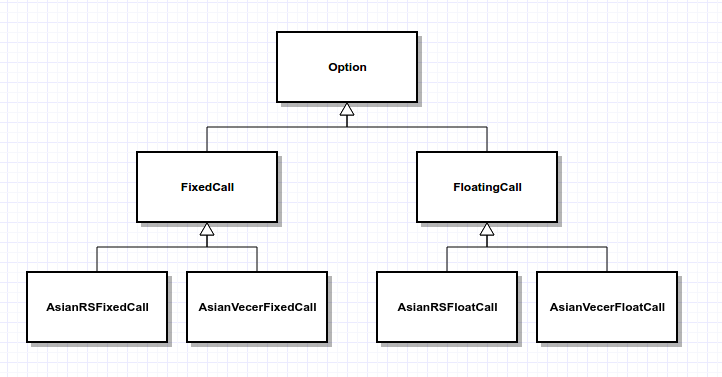
\includegraphics[width=\textwidth]{class_diagram}
  \end{frame}

  \begin{frame}
    \frametitle{Option class}
    \begin{itemize}
      \item State Variables
      \begin{itemize}
        \item \(T\)
        \item Number of points for \(\xi\)
        \item Number of points for \(t\)
        \item \(r\)
        \item \(\sigma\)
        \item \(S_0\)
        \item \(A\)
        \item \(t_0\)
        \item \(\Delta t\)
      \end{itemize}
    \end{itemize}
  \end{frame}

  \begin{frame}
    \frametitle{Option class}
    \begin{itemize}
      \item Implemented Methods
      \begin{itemize}
        \item \(q(t)\)
        \item \(A_t\)
        \item \texttt{set\_boundary\_conditions}
        \item \texttt{set\_bottom\_boundary}
        \item \texttt{set\_top\_boundary}
        \item \texttt{set\_initial\_boundary}
        \item \texttt{A\_matrix}
        \item \texttt{B\_matrix}
        \item \texttt{solve}
      \end{itemize}
    \end{itemize}
  \end{frame}

  \begin{frame}
    \frametitle{Option class}
    \begin{itemize}
      \item Abstract methods
      \begin{itemize}
        \item \texttt{alpha}
        \item \texttt{beta}
        \item \( a(t) \)
        \item \( b(t) \)
        \item \texttt{initial\_value\_at\_top}
        \item \texttt{initial\_value\_at\_bottom}
        \item \texttt{initial\_value\_at\_height}
        \item \(\xi_t\)
      \end{itemize}
    \end{itemize}
  \end{frame}

  \begin{frame}
    \frametitle{Important sub-classes}
    Both the following key classes implement \(\xi_t\), and in the fixed call case, keeps the strike as a state variable.
    \begin{itemize}
      \item \texttt{FixedCall}
      \item \texttt{FloatingCall}
    \end{itemize}
    Since then most of the methods are inherited from the base \texttt{Option} class, each method of pricing is only requred to implement the abstract methods as applicable, i.e. each PDE can be implemented in as few as 30 lines of code.
  \end{frame}

  \section{Example 1: Rogers-Shi Fixed Strike}

  \begin{frame}
    \frametitle{Rogers-Shi equation for Fixed Strike Asian Calls}
    We take
    \begin{equation}
      \xi_t = q(t)e^{(r-\delta)(T-t)} - e^{(r-\delta)(T-t)}\frac{A_t - Ke^{-\delta(T-t)}}{\tilde{S_t}}.
    \end{equation}

    Then, we have \( a(t) = -q(t)b(t) \) and \(b(t) = -e^{-(r-\delta)(T-t)}\). The partial differential equation then becomes

    \begin{equation}
      \phi_t - ( (r-\delta)\xi + \frac{1}{t_0 + T} ) \phi_\xi + \frac{1}{2}\sigma^2\xi^2\phi_{\xi\xi} = 0.
    \end{equation}
  \end{frame}

  \begin{frame}
    \frametitle{Rogers-Shi equation for Fixed Strike Asian Calls}
    Rogers and Shi show that the value of the option at time \(t\) is given by \(S_t\phi(t, \xi_t)\). We then solve the PDE with the following conditions:

    \begin{equation}
      \phi(T, \xi) = 0, 0 \le \xi \le \xi_{max}
    \end{equation}
    \begin{equation}
      \phi(t, 0) = q(t)
    \end{equation}
    \begin{equation}
      \phi(t, \xi_{max}) = 0, 0 \le t \le T.
    \end{equation}
  \end{frame}

  \begin{frame}
    \frametitle{Transformed PDE}
    This problem is transformed with \(\tau = T - t \), such that \(\psi(\tau, \xi) = \phi(T-\tau, \xi)\). This changes our partial differential equation to
    \begin{equation}
      \psi_\tau = \frac{1}{2}\sigma^2\xi^2\psi_{\xi\xi} - (r\xi + \frac{1}{T})\psi_\xi,
    \end{equation}
    subject to the conditions
    \begin{equation}
      \psi(0, \xi) = 0, 0 \le \xi \le \xi_{max},
    \end{equation}
    \begin{equation}
      \psi(\tau, 0) = \frac{1-e^{-r\tau}}{rT},
    \end{equation}
    \begin{equation}
      \psi(\tau, \xi_{max}) = 0, 0 \le \tau \le T.
    \end{equation}
  \end{frame}

  \begin{frame}
    We let \(\Delta\tau = \frac{T}{n}\) and \(\Delta\xi = \frac{\xi_{max}}{m}\), and define \(0 \le i \le n\) and \(0 \le j \le m\) as the indexes required for the finite difference grid.

    Replacing the PDE with the Crank-Nicholson discretizations yields the following equation:
    \begin{equation}
      \begin{split}
        \frac{u_{i+1, j} - u_{i, j}}{\Delta\tau} = & \frac{1}{2}\sigma^2j^2(\Delta\xi)^2 * \frac{u_{i, j+1} - 2u_{i, j} + u_{i, j-1} -2u_{i+1, j} + u_{i+1, j-1}}{2(\Delta\xi)^2} \\ & - (rj\Delta\xi + \frac{1}{T}) * \frac{u_{i, j+1} - u_{i,j-1} +u_{i+1, j+1} - u_{i+1, j-1}}{4\Delta\xi}.
      \end{split}
    \end{equation}
  \end{frame}

  \begin{frame}
    \frametitle{Abstraction}
    We extract out the common variables such that
    \begin{equation}
      \alpha(j) = \frac{1}{4}\sigma^2j^2\Delta\tau,
    \end{equation}
    \begin{equation}
      \beta(j) = \frac{1}{4\Delta\xi}\Delta\tau(rj\Delta\xi - \frac{1}{T}).
    \end{equation}
  \end{frame}

  \begin{frame}
    \frametitle{Final Discretization}
    The discretization is rearranged to yield
    \begin{equation}
      \begin{split}
        u_{i+1, j} = & (1-2\alpha(j))u_{i, j} \\
        & + (\alpha(j)-\beta(j))u_{i, j+1}\\
        & + (\alpha(j)+\beta(j))u_{i, j-1}\\
        & + (-2\alpha(j))u_{i+1, j}\\
        & + (\alpha(j)-\beta(j))u_{i+1, j+1}\\
        & + (\alpha(j)+\beta(j))u_{i+1, j-1}.
      \end{split}
    \end{equation}
  \end{frame}

  \begin{frame}
    \frametitle{Matrix form}
    We convert to the matrix form required for the Implicit Difference Scheme used.

    \begin{equation}
      \textbf{r} = \textbf{Al} + \textbf{Br},
    \end{equation}

    where

    \begin{equation}
      \textbf{l} = u_{i},
    \end{equation}
    \begin{equation}
      \textbf{r} = u_i+1,
    \end{equation}

    rearranged to yield

    \begin{equation}
      \textbf{(I-B)}\textbf{r} = \textbf{Al}
    \end{equation}

  \end{frame}

  \begin{frame}
    \frametitle{Matrix form}
    \tiny
    \begin{equation}
      \textbf{A} = \begin{bmatrix}
        1-2\alpha(0) & \alpha(0) - \beta(0) & 0 & 0 & \hdots & 0 \\
        \alpha(1) + \beta(1) & 1-2\alpha(1) & \alpha(1) - \beta(1) & 0 & \hdots & 0 \\
        0 & \alpha(2) + \beta(2) & 1-2\alpha(2) & \alpha(2) - \beta(2) & \hdots & 0 \\
        \vdots & \vdots & \vdots & \vdots & \ddots & \vdots \\
        0 & 0 & 0 & 0 & \hdots & 1-2\alpha(m)
      \end{bmatrix},
    \end{equation}
    \begin{equation}
      \textbf{B} = \begin{bmatrix}
        -2\alpha(0) & \alpha(0) - \beta(0) & 0 & 0 & \hdots & 0 \\
        \alpha(1) + \beta(1) & -2\alpha(1) & \alpha(1) - \beta(1) & 0 & \hdots & 0 \\
        0 & \alpha(2) + \beta(2) & -2\alpha(2) & \alpha(2) - \beta(2) & \hdots & 0 \\
        \vdots & \vdots & \vdots & \vdots & \ddots & \vdots \\
        0 & 0 & 0 & 0 & \hdots & -2\alpha(m)
      \end{bmatrix}.
    \end{equation}
  \end{frame}

  \begin{frame}
    \frametitle{Implementation}
    We can then proceed with solving the Finite Difference Grid based on the above recurrence relation. Adjusting \(\xi_{max}\) such that we have

    \begin{equation}
      \xi_{max} = \frac{3K}{S_0}.
    \end{equation}

    We select \(j'\) such that

    \begin{equation}
      j' = round(\frac{K}{S_0\Delta\xi}).
    \end{equation}

    Then, the fair price of the option \(P\) is given by

    \begin{equation}
      P = S_0 u_{n, j'}
    \end{equation}
  \end{frame}

  \begin{frame}[fragile]
    \frametitle{Implementation}
    \tiny
    \lstset{ %
      language=Python,
      breaklines=true,
      otherkeywords={self},             % Add keywords here
      keywordstyle=\color{deepblue},
      emph={__init__},          % Custom highlighting
      emphstyle=\color{deepred}    % Custom highlighting style
    }
    \begin{lstlisting}
class AsianRSFixedCall(FixedCall):
    def __init__(self, maxt, numx, numt, r, sigma, initial_price, strike):
        super().__init__(maxt, numx, numt, r, sigma, initial_price, strike)
        self.j0 = round(numx/3)
        self.dx = self.strike / self.s0 / self.j0
        self.maxx = numx * self.dx
        self.set_boundary_conditions()
    def initial_value_at_bottom(self, time):
        return (1 - math.exp(-self.r * time * self.dt)) / (self.r * self.maxt)
    def a(self, t):
        return -self.q(t) * self.b(t)
    def b(self, t):
        return -math.exp(self.r*(self.maxt - t))
    def alpha(self, height, time):
        return .25 * self.sigma**2 * height**2 * self.dt
    def beta(self, height, time):
        return (height * self.r * self.dx + 1 / self.maxt) * self.dt  / (4 * self.dx)
    def A_matrix(self):
        return super().A_matrix(0, lambda a, b: a + b, lambda a, b: 1 - 2*a, lambda a, b: a - b)
    def B_matrix(self):
        return super().B_matrix(0, lambda a, b: a + b, lambda a, b: -2 * a, lambda a, b: a - b)
    def solve(self):
        self.fake_super_solve(lambda time: numpy.identity(self.numx + 1) - self.B_matrix(), lambda time: self.A_matrix())
        return self.s0 * self.grid[self.j0, self.numt]
    \end{lstlisting}
    % Indenting this next line breaks the build (latex seriously?)
\end{frame}

  \section{Results}

  \begin{frame}
    \frametitle{Results for Fixed Strike Calls}
    \small
    \begin{table}[h]
      \begin{tabular}{|c|c|c|c|c|c|c|c|}
      \hline
      Volatility & Strike & Benchmark & RS & Vecer & DL & New & New-Vecer \\
      \hline
      0.05 & 90 & 13.38 & 12.91 & 13.39 & 13.38 & 6.51 & 13.38 \\
      0.05 & 95 & 8.81 & 7.84 & 8.61 & 8.81 & 3.86 & 8.81 \\
      0.05 & 100 & 4.31 & 3.65 & 4.37 & 4.27 & 1.71 & 4.31 \\
      0.05 & 105 & 0.96 & 1.37 & 0.89 & 0.96 & 0.6 & 0.95 \\
      0.05 & 110 & 0.05 & 0.44 & 0.06 & 0.08 & 0.18 & 0.06 \\
      0.1 & 90 & 13.39 & 12.7 & 13.4 & 13.38 & 6.41 & 13.39 \\
      0.1 & 95 & 8.91 & 8.22 & 8.72 & 8.91 & 4.07 & 8.91 \\
      0.1 & 100 & 4.92 & 4.48 & 4.96 & 4.89 & 2.16 & 4.91 \\
      0.1 & 105 & 2.07 & 2.08 & 2 & 2.07 & 0.97 & 2.06 \\
      0.1 & 110 & 0.63 & 0.85 & 0.65 & 0.64 & 0.38 & 0.63 \\
      0.6 & 90 & 19.96 & 19.02 & 19.91 & 19.93 & 9.81 & 19.96 \\
      0.6 & 95 & 17.41 & 16.62 & 17.26 & 17.38 & 8.54 & 17.41 \\
      0.6 & 100 & 15.13 & 14.48 & 15.14 & 15.11 & 7.42 & 15.13 \\
      0.6 & 105 & 13.11 & 12.57 & 13.04 & 13.11 & 6.42 & 13.11 \\
      0.6 & 110 & 11.34 & 10.89 & 11.37 & 11.34 & 5.55 & 11.34 \\
      \hline
      \end{tabular}
    \end{table}
  \end{frame}

  \begin{frame}
    \frametitle{Results for Floating Strike Calls}
    \scriptsize
    \begin{table}[h]
      \begin{tabular}{|c|c|c|c|c|c|c|c|c|}
      \hline
      Volatility & t0 & Average & Benchmark & RS & Vecer & DL & New & New-Vecer \\
      \hline
      0.3 & 0.1 & 90 & 9.86 & 9.86 & 9.86 & 9.89 & 9.86 & 10.45 \\
      0.3 & 0.1 & 100 & 9.35 & 9.34 & 9.33 & 9.38 & 9.35 & 9.8 \\
      0.3 & 0.1 & 110 & 8.85 & 8.85 & 8.85 & 8.88 & 8.85 & 9.21 \\
      0.3 & 0.7 & 90 & 11.19 & 11.19 & 11.18 & 11.19 & 11.41 & 12.33 \\
      0.3 & 0.7 & 100 & 6.86 & 6.86 & 6.85 & 6.86 & 6.96 & 7.02 \\
      0.3 & 0.7 & 110 & 3.86 & 3.86 & 3.86 & 3.87 & 3.76 & 3.7 \\
      0.5 & 0.1 & 90 & 14.09 & 14.08 & 14.08 & 13.53 & 14.08 & 14.93 \\
      0.5 & 0.1 & 100 & 13.65 & 13.64 & 13.64 & 13.49 & 13.65 & 14.33 \\
      0.5 & 0.1 & 110 & 13.23 & 13.22 & 13.23 & 13.19 & 13.22 & 13.76 \\
      0.5 & 0.9 & 90 & 11.91 & 11.91 & 11.91 & 11.91 & 12.04 & 13.2 \\
      0.5 & 0.9 & 100 & 6.44 & 6.44 & 6.44 & 6.43 & 6.38 & 6.5 \\
      0.5 & 0.9 & 110 & 3.05 & 3.05 & 3.04 & 3.05 & 2.87 & 2.82 \\
      \hline
      \end{tabular}
    \end{table}
  \end{frame}

\end{document}
